\graphicspath{Figures/sus13009}

\chapter{Results and Interpretation}
\label{chap:sus13009results}

\chapterquote{Physics, as we know it, will be over in six months.}
{(1928) Max Born, 1882 -- 1970}


We show the results and interpretations of a search for events containing a single energetic jet and missing transverse momentum, 
using a data sample collected at 8~\TeV by the \ac{CMS} detector at the \ac{CERN} \ac{LHC} and corresponding to an integrated luminosity of 19.7~\fbinv.
In this chapter, we show the results of the search described in Chapter~\ref{chap:sus13009} and interpret these in the context of \ac{SMS} of \ac{SUSY} in the third generation.




%
\section{Signal MC simulation} 
\label{sec:GEN}

Signal MC are Simplified Model Spectra (SMS)~\cite{bib:SMS}. 
The use of SMS samples allows one to quantify the dependence of experimental limits in a more general way, compared to a Constrained Minimal Supersymmetric Scenario (CMSSM). 
Signal samples were generated using \textsc{MadGraph 5} and showered with \textsc{Pythia 6} with up to 2 partons, and the CMS detector response simulated using the CMSSW FastSim prescription.
The MLM matching prescription is used to avoid double counting between the matrix element calculations and parton showering.
Stop and sbottom production Cross sections are taken from the LHC SUSY Cross Section Working Group \cite{bib:SUSYxs}.

Stop signal simulation 
contains events where pair produced stops decay to a charm-neutralino pair with 100\% branching fraction
in the ($m_{\sTop}, m_{\sTop} - m_{\chiOneZero}$) mass plane from $m_{\sTop} =$100~\GeV to 350~\GeV in steps of 25~\GeV, and 
$m_{\sTop} - m_{\chiOneZero} = $ 10, 20, 30, 40, 60, and 80~\GeV. 
There are two additional points at  $m_{\sTop} =$250, 275~\GeV and $m_{\sTop} - m_{\chiOneZero} = $ 5 to probe the monojet limit towards stop-neutralino degeneracy.
An additional set of stop events at $m_{\sTop} =$ 200~\GeV and $m_{\sTop} - m_{\chiOneZero} =$ 10, 80~\GeV were showered with up to 3 partons.
The difference in signal acceptance between the 2-parton and 3-parton samples
is found to be small; a table of acceptances for both samples can be found in Appendix~\ref{app:2_3_jetCutFlows}, 
which shows at $\Delta M = 10$~\GeV, there is $<1\%$ difference between the two showering methods.

An additional interpretation of pair produced sbottom quarks, which both decay to a bottom-neutralino pair 
with 100\% branching fraction is also investigated.
These SMS sbottom signal samples are produced in the same way as the stop samples; with a larger range of phase space covered. 
Here, we analyse
$m_{\sBot} =$100~\GeV to 450~\GeV in steps of 25~\GeV, and 
$m_{\chiOneZero} = $ 1, 50, 100...~\GeV, for $m_{\chiOneZero} < m_{\sBot}$.
There are also points generated along the degeneracy line, at 
$m_{\sBot} - m_{\chiOneZero} = 10$~\GeV.


`

\section{Results}
A summary of the predictions and corresponding uncertainties for all the SM backgrounds compared to the data are shown in Table~\ref{tab:summary_bgd}.
No significant deviation from the standard model is observed.


\begin{table*}%[!Hhtb]  %table 8   110811:05  
        \begin{center}
\caption{Summary of the SM background predictions and their corresponding uncertainties compared to the data.}
\label{tab:summary_bgd}
\footnotesize
                \begin{tabular}{l|lllllll} \hline
$\pt(\,\mathrm{j}_1)$ (\GeV)   &  $> 250$ &   $> 300$ &  $> 350$ &  $> 400$ &  $> 450$ &  $> 500$ &  $> 550$  \\ \hline
\znunu\,+\,jets&21209$\pm$1115  & 10077$\pm$592   & 4597$\pm$324  & 2250$\pm$197  & 1250$\pm$137  & 663$\pm$94    & 334$\pm$65 \\  
W\,+\,jets                            &12328$\pm$707   & 5939$\pm$366    & 2690$\pm$180  & 1246$\pm$92   & 627$\pm$52    & 301$\pm$29    & 150$\pm$18 \\ 
\ttbar                            &602$\pm$301     & 344$\pm$172     & 178$\pm$89    & 91$\pm$46     & 48$\pm$24     & 27$\pm$14     & 18$\pm$9.0 \\
\zellell\,+\,jets    &127$\pm$64      & 75$\pm$38       & 40$\pm$20     & 25$\pm$13     & 17$\pm$8.3    & 11$\pm$5.6    & 7.4$\pm$3.7\\
Single top                          &172$\pm$86      & 97$\pm$49       & 49$\pm$24     & 21$\pm$10     & 11$\pm$5.7    & 5.2$\pm$2.6   & 3.2$\pm$1.6\\
QCD Multijets                     &786$\pm$473     & 508$\pm$306     & 304$\pm$184   & 162$\pm$99    & 80$\pm$49     & 52$\pm$32     & 28$\pm$18  \\
Diboson                           &639$\pm$320     & 369$\pm$184     & 206$\pm$103   & 113$\pm$56    & 64$\pm$32     & 36$\pm$18     & 21$\pm$10  \\ \hline
Total SM                          &35862$\pm$1474  & 17409$\pm$803   & 8064$\pm$437  & 3907$\pm$250  & 2098$\pm$160  & 1096$\pm$106  & 563$\pm$71 \\
Data                              &36582           & 17646           & 8119          & 3896          & 1898          & 1003          & 565        \\ \hline

       \end{tabular}                                                                                   
\end{center}
\end{table*}



\section{Systematic Uncertainties on Signal}
\label{sec:SYST}
The systematic uncertainties on the background event yields have been described in detail in the previous section. 
The dominant source of uncertainty on the signal is from uncertainty due to ISR modelling.

The selection of signal events (and therefore the signal acceptance) in this analysis relies on a high-\pt ISR jet, so the modelling of ISR must be reliable.
The predicted and measured \pt spectra of recoiling systems against ISR jets is studied in~\cite{CMSsinglelep} for Z\,+\,jets, 
\ttbar and other processes. 
The simulation is found to over predict the data by 20\% for ISR jets with $\pt > 250$ \GeV.
All signal acceptances have been weighted by a factor of 0.8 to correct for this difference between data and simulation.
The uncertainty due to mismodelling of ISR jets is assigned 20\% to account for this difference for the high \pt ISR jets involved.


Other sources of uncertainty considered are:
\begin{itemize}
  \item jet energy scale (JES), emulated by shifting the jet 4-vector 
   by an $\eta$ and $\pt$ dependent factor related to the 
   response.  After these corrections, the uncertainty due to the energy scale of these corrected jets on signal acceptance using a representative signal point was found to be 5$\%$.
 In addition, a cross-check of the Jet and $\MET$ energy scale for the monojet topology is performed using \zmumu events. A detailed description of this cross-check can be found in Appendix~\ref{appendix_met_energyscale}. The $\MET$ scale derived using this method is found to be consistent with that from the recommended JES uncertainty. 
  \item uncertainties on the parton density function. The PDF uncertainty for a representative signal sample was found to be less than 2$\%$. 
  \item the difference in acceptance that is obtained from generating signal events with up to 3 partons in \MADGRAPH rather than 2 partons ($<4\%$ for $\pt(\,\mathrm{j}_1) > 500~\GeV$). 
\end{itemize}

The total uncertainty on the signal is taken to be a conservative 25$\%$.
The error on the luminosity measurement is 2.6\% ~\cite{lumi:Summer2013}.


\section{Interpretation and exclusion limits}
\label{sec:STAT}

To interpret the consistency of the observed number of events with
the background expectation in the context of a model, and also to
facilitate comparison with previous results, we set limits on the production cross section of top and bottom squarks as a function of the top and bottom squark mass and the LSP mass. 


The CL$_{s}$ method is used to estimate a 95\% credible interval limit for a signal cross section in a counting experiment~\cite{bib:STAT_RooStats,bib:BKG_PDG}.
Given the integrated luminosity, signal acceptance, background expectation and number of observed events (with associated uncertainties),
the 95\% CL upper limit on the signal cross section is set.
The theory top squark production cross sections, equal to the bottom squark production cross sections, and $\pm1\sigma_{\rm theory}$ bands are from a collaboration between the ATLAS, CMS
and LPCC SUSY working groups. Theory uncertainties are dominated by PDF uncertainties 
and calculations are detailed in \cite{bib:SUSYxs}. 

Expected limits are calculated as a function of $\pt(\,\mathrm{j}_1)$ for every ($m_{\sTop}, m_{\chiOneZero}$) or ($m_{\sBot}, m_{\chiOneZero}$) using the background expectation in each signal region. 
The signal region where the best (i.e. lowest) expected limit is found is selected as the optimal region in which to set limits for that mass point.
A fluctuation in the number of $Z(\mu\mu)$ events at $\pt(\,\mathrm{j}_1)>450$~\GeV means we have discounted this bin from the limit setting procedure in order to smooth 
the curves out.

The expected limits for each mass point in the stop, LSP mass plane at every $\pt(\,\mathrm{j}_1)$ bin can be found in Figure~\ref{fig:opt_DM}. 
The temperature plots in Figure~\ref{fig:optimalJ1} show the best expected limit across the phase space range for both stop, LSP mass planes and sbottom, LSP mass planes. 
%
Figure~\ref{fig:stop_limits} shows the expected and observed limits on the stop production cross section for the optimised $\pt(\,\mathrm{j}_1)$ bin, 
as a function of the top squark mass for mass differences between the top squark and LSP ($m_{\sTop} - m_{\chiOneZero}$) 
of $10, 20, 30, 40, 60$ and  $80~\GeV$. 
Figure~\ref{fig:sbottom_limits} shows the optimised expected and observed limits for various bottom squark masses as a function of mass difference, $m_{\sBot} - m_{\chiOneZero}$.
Figure~\ref{fig:stop_limits_2D} shows 95\% CL expected $\pm 1 \sigma_{\rm exp}$ and observed limits $\pm 1 \sigma_{\rm theory}$ on the top squark production cross section 
as a function of top squark mass and LSP mass, and top squark mass and $\Delta M$. 
The observed and expected limits on the stop production cross section are also tabulated in Tables~\ref{tab:expected_limits} and~\ref{tab:observed_limits}. 

Figure~\ref{fig:sbottom_limits_2D} shows the 95\% CL expected $\pm 1 \sigma_{\rm exp}$ and observed limits $\pm 1 \sigma_{\rm theory}$ on the bottom squark production cross section 
as a function of bottom squark mass and LSP mass.
The region of compressed phase space from approximately $m_{\sBot}=275~\GeV$, $m_{\sBot} - m_{\chiOneZero}=0$~\GeV to $m_{\sBot}=165~\GeV$, $m_{\sBot} - m_{\chiOneZero} = 85 $~\GeV is excluded at 95\% CL. 
This limit is from `monojet'-like events, that are boosted such that an ISR jet is radiated and balances the \pt of LSPs leaving the detector (giving rise to \MET).
The region of phase space from approximately $m_{\sBot}=165~\GeV$, $m_{\chiOneZero} = 40$~\GeV to $m_{\sBot}=275~\GeV$, $m_{\chiOneZero} = 0$~\GeV is also excluded.
Here, dijet events dominate; the N$_{jet} \leq 2$ requirement allows for events in which two jets, originating from the bottom quark decay products, passing the event selection. 
At least of these b-jets must be very energetic, above the optimal \pt threshold of that point of phase space. If there are two jets in the event, either the other b-jet or an ISR jet, it must be above 60~\GeV. Again, the \MET in these events arises from boosted LSPs leaving the detector, only now they are balanced by the momenta of the b-jets.
Figure~\ref{fig:sbottom_limits_2D} also shows that bottom squarks are excluded for $m_{\sBot} < 165~\GeV$ for all LSP masses. 


\begin{figure}[!Hhtb]
  \begin{center}
  \includegraphics[scale=0.39]{Figures/sus13009/limits/optimisation_Limit_10.pdf}
  \includegraphics[scale=0.39]{Figures/sus13009/limits/optimisation_Limit_20.pdf}
  \includegraphics[scale=0.39]{Figures/sus13009/limits/optimisation_Limit_30.pdf}
  \includegraphics[scale=0.39]{Figures/sus13009/limits/optimisation_Limit_40.pdf}
  \includegraphics[scale=0.39]{Figures/sus13009/limits/optimisation_Limit_60.pdf}
  \includegraphics[scale=0.39]{Figures/sus13009/limits/optimisation_Limit_80.pdf}
  \caption{Expected limit as a function of $\pt(j_{1})$\GeV.}
  \label{fig:opt_DM}
  \end{center}
\end{figure}

\begin{figure}[!Hhtb]
  \begin{center}
  \includegraphics[scale=0.39]{Figures/sus13009/limits/optimalLimits.pdf}
  \includegraphics[scale=0.39]{Figures/sus13009/sbottomlimits/optimal_jet1pT.pdf}
  \caption{The temperature plot shows the $\pt(\,\mathrm{j}_1)$ threshold at which the best expected limit is found, as a function of $m_{\sTop}$, and $m_{\sTop} - m_{\chiOneZero}$ (left) and $m_{\sBot}$ and $m_{\chiOneZero}$ (right).}
  \label{fig:optimalJ1}
  \end{center}
\end{figure}



%The results of the monojet search can also be interpreted to constrain the production of light stops. The observed limits on the production cross section as a function of the stop mass are shown in Figure~\ref{fig:stop_limits} for mass splittings of 10 GeV, 30 GeV and 80 GeV. Also shown are the expected limits and the theoretical prediction. The observed (expected) limits on the stop mass for the 10 GeV and 30 GeV mass splitting are; 250 (255) GeV and 190 (195) GeV respectively.
\begin{figure}[!Hhtb]
  \begin{center}
%  \includegraphics[scale=0.39]{m10.pdf}
%  \includegraphics[scale=0.39]{m30.pdf}
  \includegraphics[scale=0.39]{Figures/sus13009/limits/Limit10.pdf}
  \includegraphics[scale=0.39]{Figures/sus13009/limits/Limit20.pdf}
  \includegraphics[scale=0.39]{Figures/sus13009/limits/Limit30.pdf}
  \includegraphics[scale=0.39]{Figures/sus13009/limits/Limit40.pdf}
  \includegraphics[scale=0.39]{Figures/sus13009/limits/Limit60.pdf}
  \includegraphics[scale=0.39]{Figures/sus13009/limits/Limit80.pdf}
  \caption{Optimised observed and expected limits on stop production cross section as a function of the stop mass for $m_{\sTop} - m_{\chiOneZero} = 10, 20, 30, 40, 60$ and 80 \GeV.}
  \label{fig:stop_limits}
  \end{center}
\end{figure}




\begin{figure}[!Hhtb]
  \begin{center}
%  \includegraphics[scale=0.39]{m10.pdf}
%  \includegraphics[scale=0.39]{m30.pdf}
  \includegraphics[scale=0.39]{Figures/sus13009/sbottomlimits/Limit_100.pdf}
  \includegraphics[scale=0.39]{Figures/sus13009/sbottomlimits/Limit_150.pdf}
  \includegraphics[scale=0.39]{Figures/sus13009/sbottomlimits/Limit_200.pdf}
  \includegraphics[scale=0.39]{Figures/sus13009/sbottomlimits/Limit_225.pdf}
  \includegraphics[scale=0.39]{Figures/sus13009/sbottomlimits/Limit_250.pdf}
  \includegraphics[scale=0.39]{Figures/sus13009/sbottomlimits/Limit_275.pdf}
  \caption{Optimised observed and expected limits on sbottom production cross section as a function of the mass difference $m_{\sBot} - m_{\chiOneZero}$, shown for $m_{\sBot} = 100, 150, 200, 225, 250$ and 275 \GeV. 
  The limits at low mass difference are due to monojet events, 
  where an event with a radiated ISR jet passes the event selection. 
  At large mass differences, we become sensitive to dijet events; events in which two b-jets from both bottom squark decays pass the event selection.}
  \label{fig:sbottom_limits}
  \end{center}
\end{figure}



\begin{figure}[!Hhtb]
  \begin{center}
%  \includegraphics[scale=0.39]{m10.pdf}
%  \includegraphics[scale=0.39]{m30.pdf}
  \includegraphics[scale=0.39]{Figures/sus13009/limits/limits_stopLSP.pdf}
  \includegraphics[scale=0.39]{Figures/sus13009/limits/limits_stopDM.pdf}
  \caption{ Observed and expected limits on stop production cross section as a function of the stop mass and LSP mass (left) and 
  as a function of the stop mass and $m_{\sTop} - m_{\chiOneZero}$ (right).}
  \label{fig:stop_limits_2D}
  \end{center}
\end{figure}


\begin{table*}%[!Hhtb]  %table 8   110811:05  
        \begin{center}  
        \renewcommand{\arraystretch}{1.5}
\caption{The expected limits on the production cross section of stops for different values of $m_{\sTop} - m_{\chiOneZero}$. 
Also shown are the +1$\sigma$ expected limits in superscript, and the -1$\sigma$ expected limits in subscript.}
\label{tab:expected_limits}
\small
                        \begin{tabular}{l|ccccccc} \hline
$\pt(\,\mathrm{j}_1)$ (\GeV)   &  $> 250$ &   $> 300$ &  $> 350$ &  $> 400$ &  $> 450$ &  $> 500$ &  $> 550$  \\ \hline
$m_{\sTop}-m_{\chiOneZero} = 10$ &  $ 82.98 \pm ^{ 115.7 }_{ 57.15 } $ &    $ 37.63 \pm ^{ 53.28 }_{ 28.11 } $ &    $ 23.89 \pm ^{ 33.84 }_{ 17.85 } $ &    $ 15.48 \pm ^{ 21.93 }_{ 11.56 } $ &    $ 11.02 \pm ^{ 17.5 }_{ 8.489 } $ &   $ 8.128 \pm ^{ 12.9 }_{ 6.259 } $ &   $ 6.148 \pm ^{ 9.758 }_{ 4.734 } $ \\ 
$m_{\sTop}-m_{\chiOneZero} = 20$ &   $ 129 \pm ^{ 178.2 }_{ 88.96 } $ &    $ 57.03 \pm ^{ 81.5 }_{ 39.17 } $ &   $ 32.37 \pm ^{ 46.33 }_{ 22.24 } $ &    $ 20.32 \pm ^{ 28.99 }_{ 13.96 } $ &    $ 14.1 \pm ^{ 20.16 }_{ 9.686 } $ &   $ 10.59 \pm ^{ 15.01 }_{ 7.916 } $ &    $ 7.658 \pm ^{ 12.11 }_{ 5.884 } $ \\ 
$m_{\sTop}-m_{\chiOneZero} = 30$ &  $ 210.1 \pm ^{ 298.7 }_{ 145 } $ &    $ 89.51 \pm ^{ 128.1 }_{ 61.5 } $ &   $ 51.35 \pm ^{ 72.03 }_{ 35.58 } $ &    $ 29.23 \pm ^{ 41.85 }_{ 20.08 } $ &    $ 19.03 \pm ^{ 26.95 }_{ 14.22 } $ &    $ 14.7 \pm ^{ 20.82 }_{ 10.98 } $ &   $ 10.62 \pm ^{ 15.04 }_{ 7.933 } $ \\ 
$m_{\sTop}-m_{\chiOneZero} = 40$ &   $ 259.8 \pm ^{ 357.1 }_{ 176.1 } $ &    $ 122 \pm ^{ 174.5 }_{ 83.85 } $ &    $ 66.71 \pm ^{ 95.04 }_{ 46.13 } $ &    $ 39.01 \pm ^{ 55.84 }_{ 26.8 } $ & $ 26.05 \pm ^{ 37.15 }_{ 17.9 } $ &   $ 18.67 \pm ^{ 26.73 }_{ 12.83 } $ &    $ 13.36 \pm ^{ 21.21 }_{ 10.29 } $ \\ 
$m_{\sTop}-m_{\chiOneZero} = 60$ &  $ 312.9 \pm ^{ 447.9 }_{ 214.6 } $ &    $ 156.1 \pm ^{ 218.8 }_{ 106.8 } $ &    $ 98.48 \pm ^{ 138.1 }_{ 68.23 } $ &    $ 54.47 \pm ^{ 78.02 }_{ 37.43 } $ &    $ 35.69 \pm ^{ 51.11 }_{ 24.52 } $ &    $ 27.33 \pm ^{ 39.08 }_{ 18.78 } $ &    $ 20.28 \pm ^{ 28.71 }_{ 15.15 } $ \\ 
$m_{\sTop}-m_{\chiOneZero} = 80$ &   $ 346 \pm ^{ 482.5 }_{ 240.3 } $ &    $ 175.4 \pm ^{ 247.4 }_{ 120 } $ &    $ 99.73 \pm ^{ 142 }_{ 69.04 } $ &    $ 62.38 \pm ^{ 89.35 }_{ 42.86 } $ &    $ 45.92 \pm ^{ 65.77 }_{ 31.55 } $ &    $ 32.57 \pm ^{ 46.64 }_{ 22.37 } $ &    $ 26.7 \pm ^{ 37.79 }_{ 19.95 } $ \\ 
%$ \Delta M = 10$ & 82.98 &  37.63 &  23.89 &  15.48 &  11.02 &  8.128 &  6.148 \\
%$ \Delta M = 20$ &  129  & 57.03  & 32.37  & 20.32  & 14.1   & 10.59  & 7.658 \\
%$ \Delta M = 30$ & 210.1 &  89.51 &  51.35 &  29.23 &  19.03 &  14.7  &  10.62 \\
%$ \Delta M = 40$ &  259.8&   122  & 66.71  & 39.01  & 26.05  & 18.67  & 13.36 \\
%$ \Delta M = 60$ & 312.9 &  156.1 &  98.48 &  54.47 &  35.69 &  27.33 &  20.28 \\
%$ \Delta M = 80$ &  346  & 175.4  & 99.73  & 62.38  & 45.92  & 32.57  & 26.7 \\ \hline
\end{tabular}
\end{center}
\end{table*}

\begin{table*}[!Hhtb]  %table 8   110811:05  
        \begin{center}
\caption{The observed limits on the production cross section of stops for different values of $m_{\sTop} - m_{\chiOneZero}$. }
\label{tab:observed_limits}
                        \begin{tabular}{l|ccccccc} \hline
$\pt(\,\mathrm{j}_1)$ (\GeV)   &  $> 250$ &   $> 300$ &  $> 350$ &  $> 400$ &  $> 450$ &  $> 500$ &  $> 550$  \\ \hline
$m_{\sTop}-m_{\chiOneZero} = 10$&  $ 87.75 $ &   $ 37.53 $ &   $ 23.83 $ &   $ 15.44 $ &   $ 8.843 $ &   $ 6.52 $ &    $ 4.931 $ \\ 
$m_{\sTop}-m_{\chiOneZero} = 20$&   $ 138.2 $ &   $ 58.6 $ &    $ 33.27 $ &   $ 20.89 $ &   $ 14.49 $ &   $ 10.57 $ &   $ 6.13 $ \\ 
$m_{\sTop}-m_{\chiOneZero} = 30$&  $ 225.2 $ &   $ 92.03 $ &   $ 54.86 $ &   $ 30.05 $ &   $ 18.99 $ &   $ 14.66 $ &   $ 10.59 $ \\ 
$m_{\sTop}-m_{\chiOneZero} = 40$&   $ 275.7 $ &   $ 125.5 $ &   $ 71.48 $ &   $ 40.1 $ &    $ 26.78 $ &   $ 19.19 $ &   $ 10.72 $ \\
$m_{\sTop}-m_{\chiOneZero} = 60$&  $ 337 $ &   $ 166.6 $ &   $ 105.2 $ &   $ 56.01 $ &   $ 36.69 $ &   $ 28.1 $ &    $ 20.22 $ \\ 
$m_{\sTop}-m_{\chiOneZero} = 80$&   $ 372.8 $ &   $ 187.3 $ &   $ 106.6 $ &   $ 64.14 $ &   $ 47.22 $ &   $ 33.48 $ &   $ 26.63 $ \\ \hline 


\end{tabular}
\end{center}
\end{table*}





\begin{figure}[!Hhtb]
  \begin{center}
  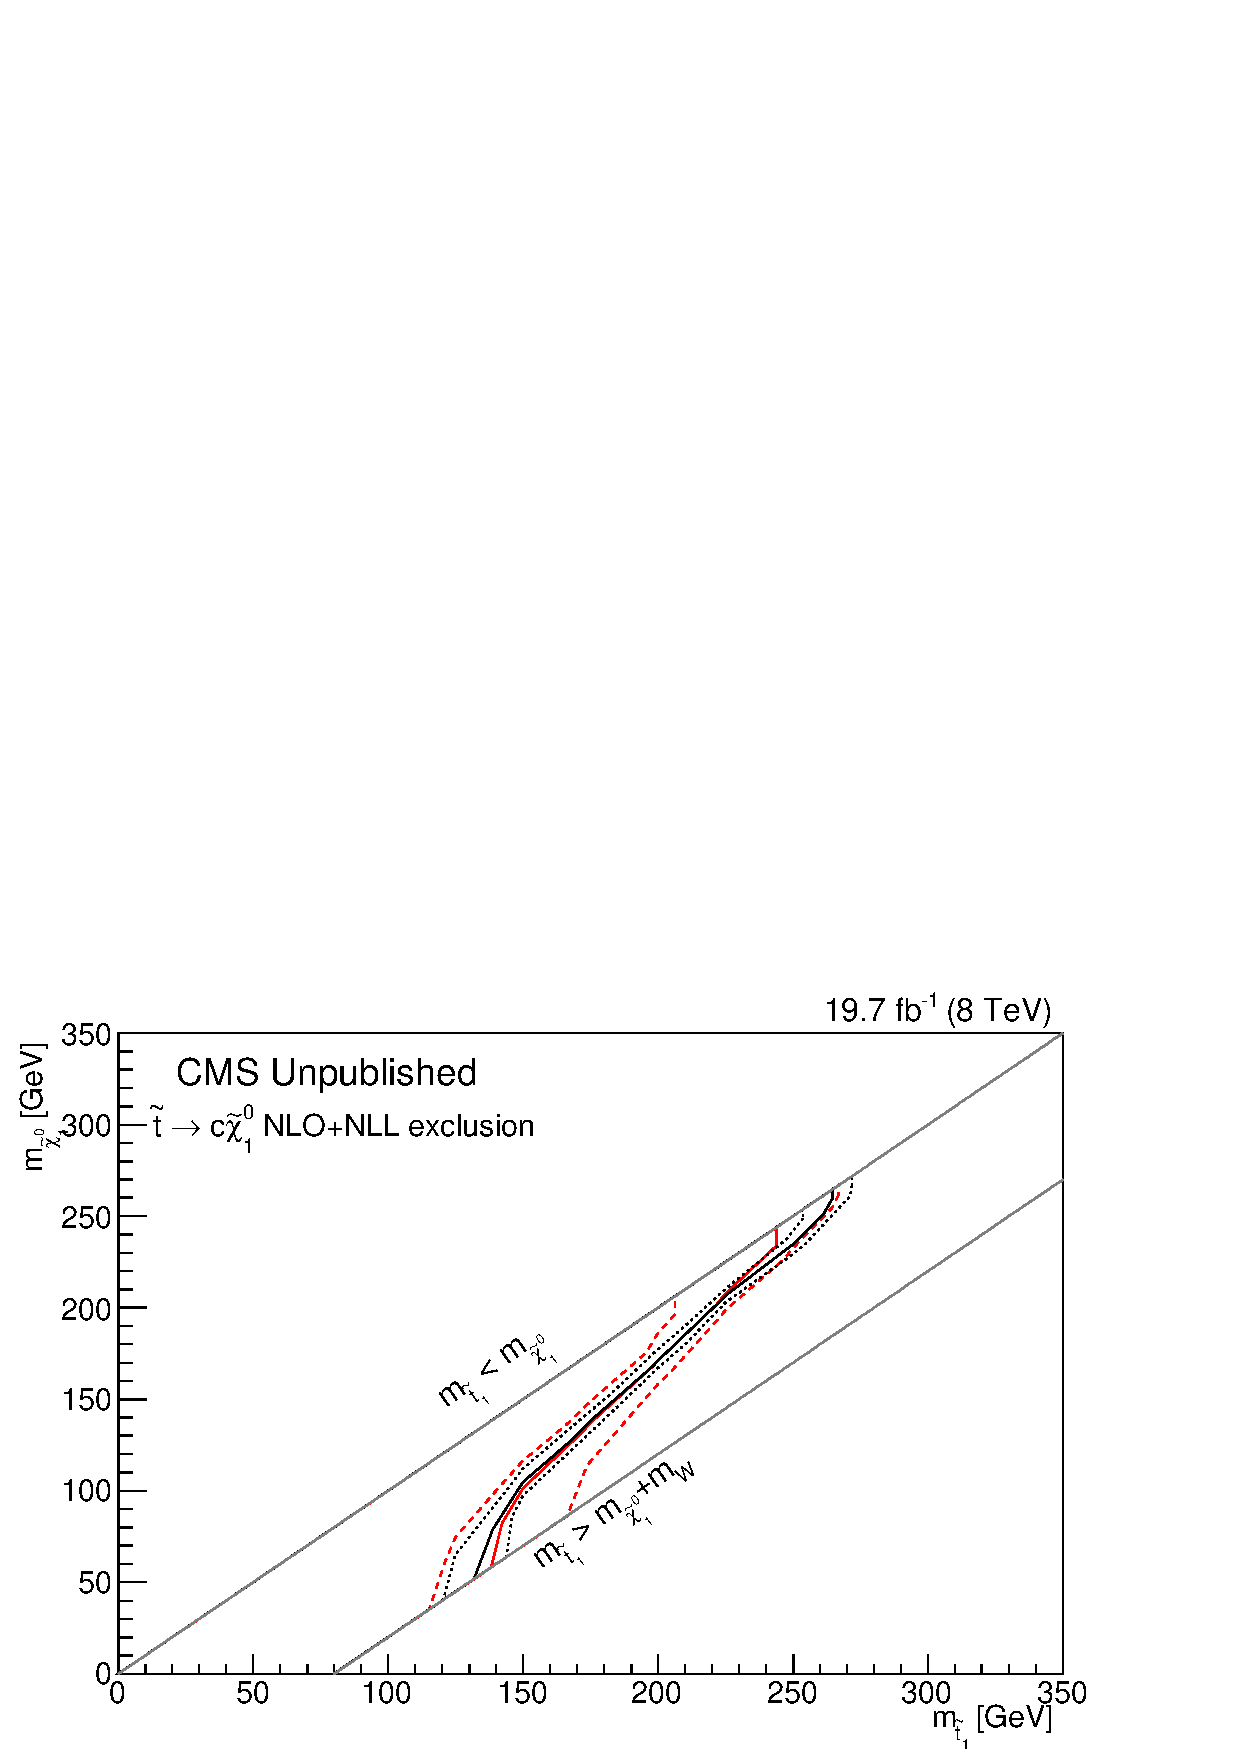
\includegraphics[scale=0.39]{Figures/sus13009/limits/mstop_lsp.pdf}
  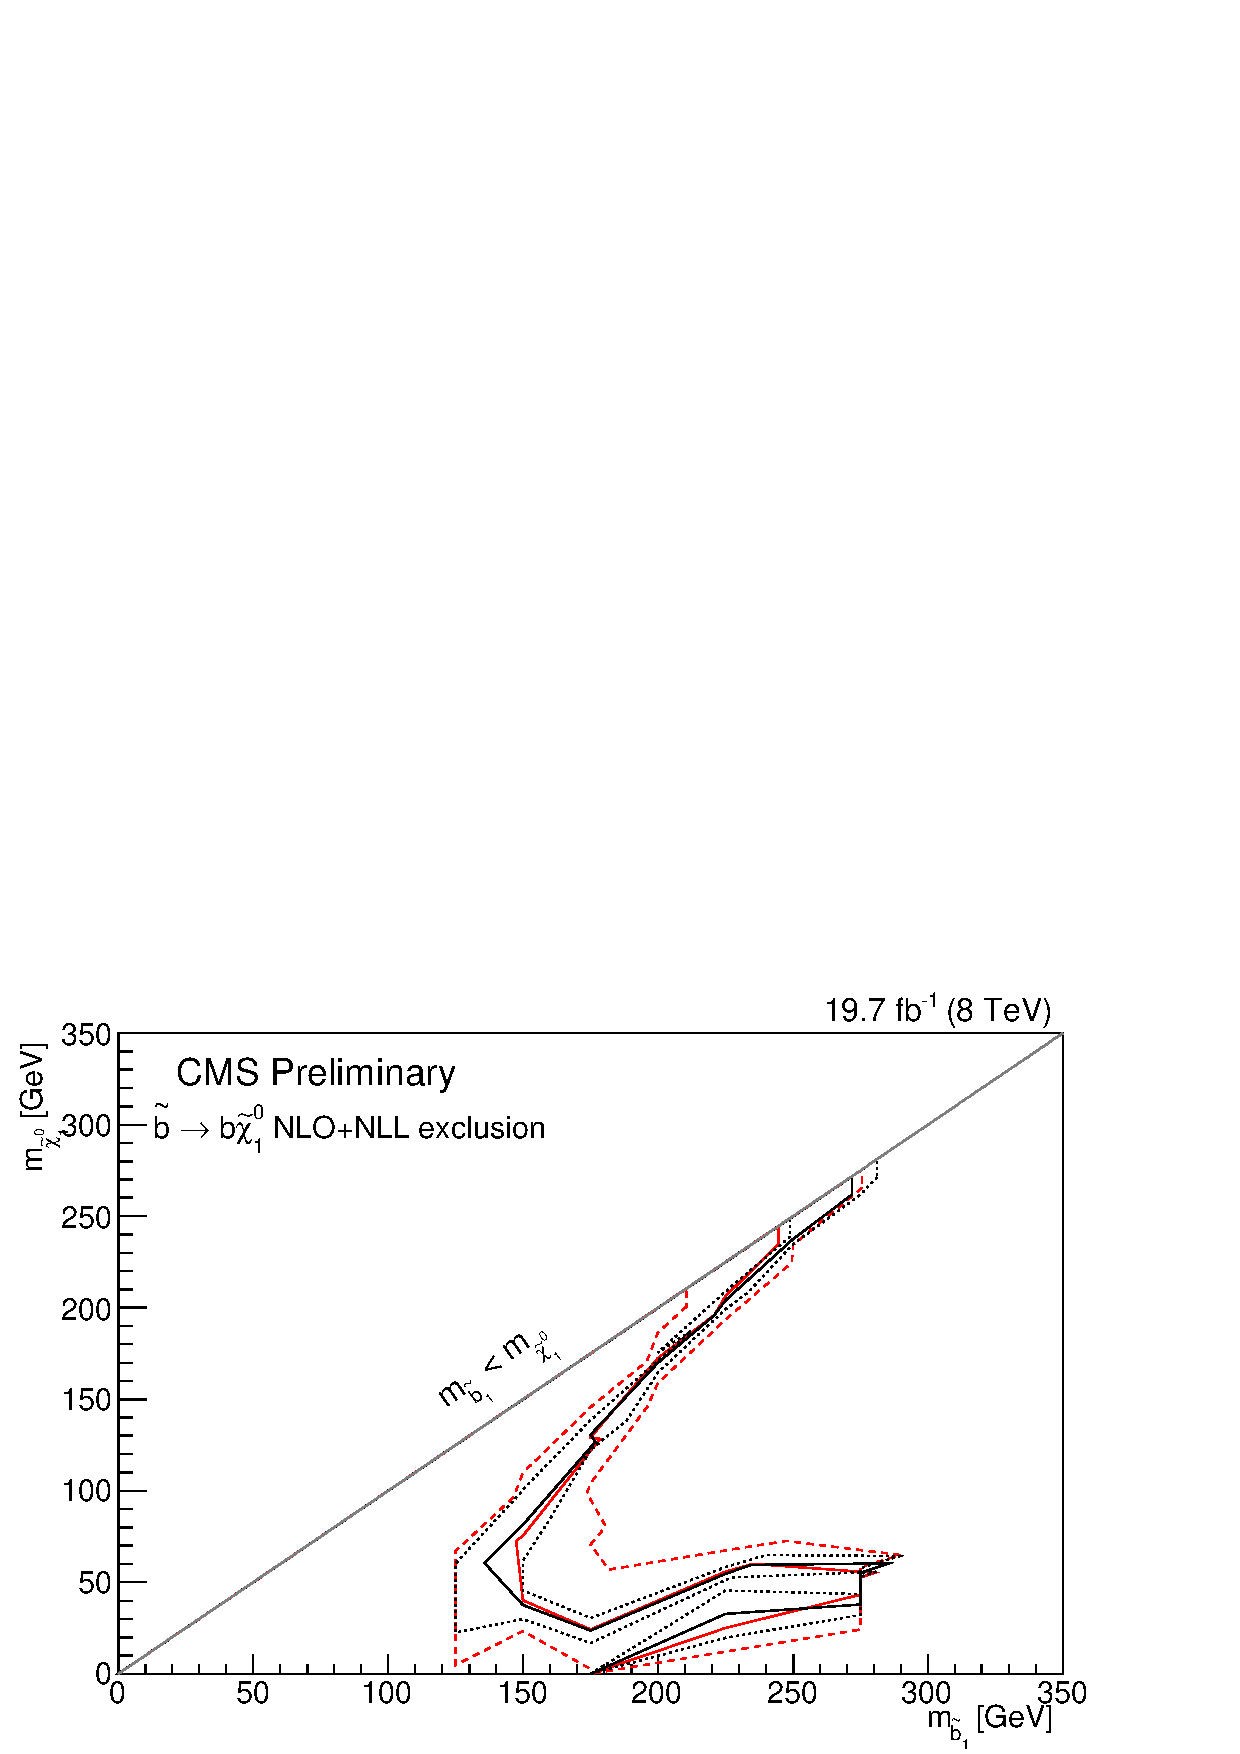
\includegraphics[scale=0.39]{Figures/sus13009/sbottomlimits/msbottom_lsp.pdf}
  \caption{ Observed and expected limits on top (left) and bottom (right) squark pair production cross section as a function of the top and bottom squark mass and LSP mass. The top squark limit is the same as the above, only formatted to allow easy comparison between the two limits, which are very similar in the compressed region, as is expected. }
  \label{fig:sbottom_limits_2D}
  \end{center}
\end{figure}




